%&pdflatex
\documentclass[tikz,border=5]{standalone}

\usetikzlibrary{arrows.meta}
\newcommand{\OO}[1]{O(#1)}

\begin{document}

\footnotesize
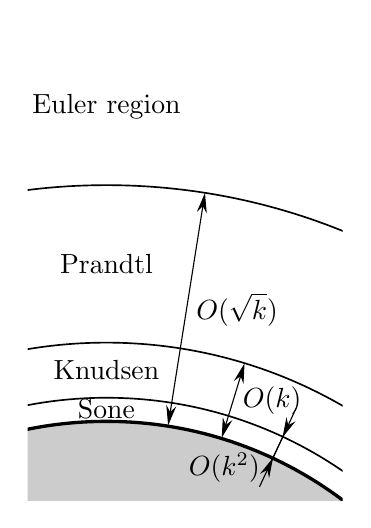
\begin{tikzpicture}[
    arrow/.style={>={Stealth[scale length=1.5]}, thin, shorten <=.3pt}
]
\pgftransformscale{2}

\clip (-0.5,2) rectangle (1.5,5);

\fill[fill=black!20, draw=black, very thick] (0,0) circle [radius=2.5];
\foreach \i in {.65,1,2}
    \draw[semithick] (0,0) circle [radius=2+\i];

\node at (0,2.58) {Sone};
\node at (0,2.83) {Knudsen};
\node at (0,3.5) {Prandtl};
\node at (0,4.5) {Euler region};

\draw[<->, arrow] (81:2.5) -- (81:4) node [right,midway] {\(\OO{\sqrt{k}}\)};
\draw[<->, arrow] (73:2.5) -- (73:3) node [right,midway] {\(\OO{k}\)};
\draw[thin] (65:2.3) node [above left=-2pt] {\(\OO{k^2}\!\)}  -- (65:2.85);
\draw[>-<, arrow, shorten <=-7pt, shorten >=-7pt] (65:2.5) -- (65:2.65) ;

\end{tikzpicture}

\end{document}
